%%%%%%%%%%%%%%%%%%%%%%% file template.tex %%%%%%%%%%%%%%%%%%%%%%%%%
%
% This is a general template file for the LaTeX package SVJour3
% for Springer journals.          Springer Heidelberg 2010/09/16
%
% Copy it to a new file with a new name and use it as the basis
% for your article. Delete % signs as needed.
%
% This template includes a few options for different layouts and
% content for various journals. Please consult a previous issue of
% your journal as needed.
%
%%%%%%%%%%%%%%%%%%%%%%%%%%%%%%%%%%%%%%%%%%%%%%%%%%%%%%%%%%%%%%%%%%%
%
% First comes an example EPS file -- just ignore it and
% proceed on the \documentclass line
% your LaTeX will extract the file if required
\begin{filecontents*}{example.eps}
%!PS-Adobe-3.0 EPSF-3.0
%%BoundingBox: 19 19 221 221
%%CreationDate: Mon Sep 29 1997
%%Creator: programmed by hand (JK)
%%EndComments
gsave
newpath
  20 20 moveto
  20 220 lineto
  220 220 lineto
  220 20 lineto
closepath
2 setlinewidth
gsave
  .4 setgray fill
grestore
stroke
grestore
\end{filecontents*}
%
\RequirePackage{fix-cm}
%
%\documentclass{svjour3}                     % onecolumn (standard format)
%\documentclass[smallcondensed]{svjour3}     % onecolumn (ditto)
\documentclass[smallextended]{svjour3}       % onecolumn (second format)
%\documentclass[twocolumn]{svjour3}          % twocolumn
%
\smartqed  % flush right qed marks, e.g. at end of proof
%
\usepackage{graphicx}
\usepackage{varwidth}
\usepackage{setspace}
%
% \usepackage{mathptmx}      % use Times fonts if available on your TeX system
%
% insert here the call for the packages your document requires
%\usepackage{latexsym}
% etc.
%
% please place your own definitions here and don't use \def but
% \newcommand{}{}
%
% Insert the name of "your journal" with
% \journalname{myjournal}
%
\begin{document}

\title{Emotion-Awareness Improves Human-Robot Collaboration}%\thanks{Grants or
% other notes about the article that should go on the front page should be
%placed here. General acknowledgments should be placed at the end of the article.}
%}

%\subtitle{Do you have a subtitle?\\ If so, write it here}

%\titlerunning{Short form of title}        % if too long for running head

\author{Mohammad Shayganfar \and
        Charles Rich \and
        Candace L. Sidner
}

%\authorrunning{Short form of author list} % if too long for running head

\institute{Mohammad Shayganfar \and Charles Rich \and Candace L. Sidner \at
              100 Institute Road, Worcester, MA, USA 01609-2280 \\
              Tel.: +1 508-831-5357\\
              Fax: +1 508-831-5776\\
              \email{mshayganfar@wpi.edu}\\
              \email{rich@wpi.edu}\\
              \email{sidner@wpi.edu}\\
%             \emph{Present address:} of F. Author  %  if needed
}

\date{Received: date / Accepted: date}
% The correct dates will be entered by the editor


\maketitle

\begin{abstract}\ldots


\keywords{Human-Robot/Agent Collaboration \and Emotion-Awareness \and Affective
Motivational Collaboration Theory}
% \PACS{PACS code1 \and PACS code2 \and more}
% \subclass{MSC code1 \and MSC code2 \and more}
\end{abstract}

\section{Introduction}
\label{intro}

\ldots

\section{Related Work}

\subsection{Emotions in Social Context}

\subsection{Social Functions of Emotions}

\subsection{Affect and Motives}

\subsection{Collaboration Theory}
\label{sec:collaboration-theory}

\section{Example Scenario}
\label{sec:1}
%Text with citations \cite{RefB} and \cite{RefJ}.

\subsection{The Backstory}

The scenario transpires in a NASA's research center. Light, temperature and
other environmental factors are simulated based on conditions on the surface of
the moon. The mission is to finish installing the required solar panels to
provide energy for the operation of NASA's science lab on the moon. Ninety
percent of these panels have already been installed. However, the operation is
now faced with low batteries which forces everyone to be cautious about
consuming energy. The astronaut is inspecting the working conditions in the
field and planning the installation of the remaining panels in collaboration
with the robot. He determines that the sun will cast shadows over the
installation structure, leading to potential difficulties. The astronaut asks
control base to go through the final checks of the robot and prepare it for the
operation.

\subsection{Astronaut-Robot Interaction}

The robot and the astronaut will collaborate with each other to achieve their
shared goal, which is to install two solar panels. They will face various
difficulties, ranging from the task being unpleasant and challenging to
conflicts of their private and/or shared goals occurring because of a blocked or
a protracted sub-task. The robot and the astronaut will go through a series of
assessment processes to figure out a) how did the current blocking happen? b)
why is the current task is blocked? and c) what is the next action they are
going to take? The robot uses its cognitive abilities and its communication
skills to overcome these problems and to motivate the astronaut to propose
alternative tasks. The following is part of an interaction between the astronaut
and the robot during their collaboration on installing solar panels.

\subsection{Agreeing on Shared Goal (Emotion-Awareness)}
\label{sec:exp1}

This and the next hypothetical examples show that agreeing on a shared goal
requires the robot to be aware of its collaborator's emotions (here it is
frustration). In this example, the Astronaut's first turn (A1), shows her
verbally conveying her frustration with respect to the disfunctioning
measurement tool for checking the quality of the installed panel. In return, the
Robot's first turn (A2), as the crucial part of this interaction shows the Robot
perceiving the Astronaut's frustration and acknowledging that verbally. Later
on, in Section \ref{sec:wt-exp1}, we are going to show how the computational
mechanisms, discussed in Section \ref{sec:AMCT}, are involved in this process.
In other words, we are going to discuss how the emotion-driven goal-directed
mechanisms can work together and lead the Robot's behavior to acknowledge
perceived emotion of the Astronaut properly to avoid termination of the
collaboration. Continuing in turn A3, the Astronaut's utterance shows the change
of the underlying belief from termination of the collaboration to a belief
showing the possibility of seeking instrumental support by asking the Robot
whether it is possible to fix the measurement tool. Notice that the proper
acknowledgement of the Astronaut's emotion helps to change her emotion from
frustration to neutral. Now that the Astronaut does not express a negative
emotion (i.e., frustration), and she is asking for instrumental support, the
Robot can provide the alternative task as a potential solution. Here is another
advantage of the emotion-awareness in this hypothetical example. Although, the
robot, according to the shared plan (see Sections \ref{sec:collaboration-theory}
and \ref{sec:AMCT}), could provide the same alternative task as solution to the
Astronaut, instead, it procrastinated providing the potential solution based on
the Astronaut's negative emotional state, i.e., frustration. Finally, since
agreeing on a shared goal is a collaborative negotiation process,
emotion-awareness plays an imperative role in providing a more fair offer to the
collaborator during negotiation. As a result, the Astronaut's response in the
last turn (A5) shows the acceptance of the Robot's potential solution to
continue collaboration and agreeing on the shared goal. In the next example we
are going to show what happens to the same hypothetical example when the Robot
ignores the Astronaut's emotion and tries to save the collaboration process from
failure.\\

\begin{spacing}{1.2}
\small{ 
\begin{description}
  \item \textit{\textbf{A1. Astronaut:}} Oh no! Finishing the quality check of
  our installation with this measurement problem is so frustrating. I think we
  should stop now!

  [\textit{Astronaut is frustrated.}]\\

  \item \fbox{\begin{varwidth}{0.96\textwidth}\textit{\textbf{A2. Robot:}}
  \underline{I see. This is frustrating.} But, I can help you with the
  measurement tool and we can finish the task as originally planned.

  [\textit{Robot perceives Astronaut's frustration and acknowledges that.}]
  \end{varwidth}}\\
  
  \item \textit{\textbf{A3. Astronaut:}} Can you fix the measurement tool?

  [\textit{Astronaut's emotion is neutral.}]\\
  
  \item \textit{\textbf{A4. Robot:}} The next task is fixing the panel and it
  needs you to prepare and attach the welding rod to your welding tool. To save
  our time, I will fetch another measurement tool while you are preparing your
  welding tool.

  [\textit{Robot perceives Astronaut's neutral emotion, and tries to negotiate
  and provide a fair offer.}]\\

  \item \textit{\textbf{A5. Astronaut:}} That would be great!
  
  [\textit{Astronaut is content.}]
  
\end{description}
}
\end{spacing}


\subsection{Agreeing on Shared Goal (Emotion-Ignorance)}
\label{sec:exp2}

This example shows that agreeing on a shared goal requires the robot to be aware
of its collaborator's frustration. Otherwise a collaborative robot will try to
maintain the status of the shared goal and prevent it from failure without
considering its collaborator's negative emotion which can be a direct result of
a type of failure in collaboration. First, the emotion-ignorant robot does not
acknowledge the Astronaut's frustration (i.e., B2 in compare to A2 in Section
\ref{sec:exp1}), since it does not perceive that. Then, while negotiating the
shared goal the robot fails to offer a potential solution based on the
Astronaut's emotional state, resulting in the failure of the negotiation during
collaboration.

\begin{spacing}{1.2}
\small{
\begin{description}
  \item \textit{\textbf{B1. Astronaut:}} Oh no! Finishing the quality check of
  our installation with this measurement problem is so frustrating. I think we
  should stop now!

  [\textit{Astronaut is frustrated.}]\\

  \item \fbox{\begin{varwidth}{0.96\textwidth}\textit{\textbf{B2. Robot:}} I can
  help you with the measurement tool, or we can terminate this task.
  \underline{What do you want me to do?}

  [\textit{Robot does not perceive Astronaut's frustration.}] \end{varwidth}}\\
  
  \item \textit{\textbf{B3. Astronaut:}} As I said the measurement tool does not
  work properly. We can not continue!

  [\textit{Astronaut is frustrated.}]\\
  
  \item \textit{\textbf{B4. Robot:}} Okay. Do you want me to fix this problem
  or terminate the task?

  [\textit{Robot does not perceive Astronaut's frustration.}]\\

  \item \textit{\textbf{B5. Astronaut:}} Can you fix my measurement tool?
  
  [\textit{Astronaut is frustrated, even more.}]\\
  
  \item \textit{\textbf{B6. Robot:}} I cannot fix your measurement tool, but I
  can fetch another one for you if you want?
  
  [\textit{Despite Astronaut's strong frustration, Robot tries to negotiate.}]\\
  
  \item \textit{\textbf{B7. Astronaut:}} No, I don't want another measurement tool!
  We don't have time for that!
  
  [\textit{Astronaut is angry.}]\\
  
  \item \fbox{\begin{varwidth}{0.96\textwidth}\textit{\textbf{B8. Robot:}} Okay.
  You want me to terminate this task. Terminating this task can influence the
  quality of installing this solar panel which can cause the mission to fail.
  Or, \underline{do you want us to work on another task?} This can help us to
  install the panel using your welding tool, but I do not know whether the
  quality of our installation will be acceptable.
  
  [\textit{Not only the Robot does not perceive Astronaut's anger, but also
  continues to negotiate the next step based on the shared plan to select proper
  action.}] \end{varwidth}}\\
  
  \item \textit{\textbf{B9. Astronaut:}} I told you we have this problem and we
  should terminate the mission! We cannot continue without the measurement tool!
  
  [\textit{Astronaut is angry.}]\\
  
\end{description}
}
\end{spacing}

\subsection{Delegation of a Task (Emotion-Awareness)}

This example shows how delegation critically depends on understanding how
worried the other collaborator is and the necessity of having sufficient time,
which play together. The emotion-ignorant robot is doing planning in its most
efficient manner (efficient because time is short): asking a lot of questions
(i.e., B2, B4, B6, B8, B10) so that it can work out the plan. But asking
questions exacerbates the Astronaut's worry, whereas when the robot knows about
the Astronaut's worriedness, it can use its own motivation mechanism to come up
with a way to alleviate that. Its methods are to exactly postpone any questions
until such time as they are critical (i.e., A2, A4).

\begin{spacing}{1.2}
\small{
\begin{description}
  \item \textit{\textbf{C1. Astronaut:}} I still have some problems with
  attaching the first panel! We do not have enough time. You should begin to
  install the second panel.

  [\textit{Astronaut is worried.}]\\

  \item \fbox{\begin{varwidth}{0.96\textwidth}\textit{\textbf{C2. Robot:}} Okay.
  \underline{Don't worry.} I can handle that.

  [\textit{Robot perceives Astronaut's worriedness and acknowledges that. Also,
  it doesn't ask the Astronaut (because of perceiving worriedness) if it is okay
  to leave the current task which was helping the Astronaut to install the first
  panel.}]\\
  
  [\textit{Robot perceives the Astronaut's request as on “open planning” (as
  oppose to specific executive) task delegation.}]\end{varwidth}}\\
  
  \item \textit{\textbf{C3. Astronaut:}} I will try to fix it asap.

  [\textit{Astronaut's is still worried.}]\\
  
  \item \textit{\textbf{C4. Robot:}} I might need to ask some questions while I
  am installing the second panel.

  [\textit{Robot perceives Astronaut's worriedness.}]\\

  [\textit{Robot checks a) dependencies of the task (a sub-task might need to be
  done by both parties), b) preconditions, c) required resources, d) possible
  future conflicts.}]\\
  
  [\textit{Robot needs to ask several questions to remove uncertainties, but
  because of the Astronaut's emotion, Robot decided to postpone questions about
  the details to when the Astronaut's answers are necessary to make progress.
  Robot modifies its utterance in a proper way.}]\\
  
  \item \textit{\textbf{C5. Astronaut:}} That's fine. Just let me know.
  
  [\textit{Astronaut is neutral.}]
  
\end{description}
}
\end{spacing}

\subsection{Delegation of a Task (Emotion-Ignorance)}

\begin{spacing}{1.2}
\small{
\begin{description}
  \item \textit{\textbf{D1. Astronaut:}} I still have some problems with
  attaching the first panel! We do not have enough time. You should begin to
  install the second panel.

  [\textit{Astronaut is worried.}]\\

  \item \fbox{\begin{varwidth}{0.96\textwidth} \textit{\textbf{D2. Robot:}}
  Okay. I can handle that. \underline{Is it okay if I leave the current task
  though?}

  [\textit{Robot does not perceive Astronaut's worriedness.}]\\
  
  [\textit{Robot perceives the Astronaut's request as on “open planning” (as
  oppose to specific executive) task delegation.}] \end{varwidth}}\\
  
  \item \textit{\textbf{D3. Astronaut:}} Yes, that's fine. I can finish it by my
  own.

  [\textit{Astronaut is still worried.}]\\
  
  \item \textit{\textbf{D4. Robot:}} Okay. But according to the plan, I need
  your help when we need to weld the panel. Will you be able to help me?

  [\textit{Robot does not perceive Astronaut's worriedness.}]\\

  [\textit{Robot checks a) dependencies of the task (a sub-task might need to be
  done by both parties), b) preconditions, c) required resources, d) possible
  future conflicts.}]\\
  
  [\textit{Robot needs to ask several questions to remove uncertainties, so it
  does, since it misses the Astronaut's negative emotion.}]\\
  
  \item \textit{\textbf{D5. Astronaut:}} Yes, I will.
  
  [\textit{Astronaut is more worried about finishing the first panel.}]\\
  
  \item \textit{\textbf{D6. Robot:}} We also need your welding tool and supplies
  as well as the measuring tool to install the second panel.
  
  [\textit{Robot does not perceive Astronaut's worriedness. So, it continues to
  ask question.}]\\
  
  \item \textit{\textbf{D7. Astronaut:}} Just let me know whenever you need
  something!
  
  [\textit{Astronaut becomes frustrated, since he thinks the Robot's questions
  are killing time.}]\\
  
  \item \textit{\textbf{D8. Robot:}} Thanks. I will. How about the conflict that
  might occur while I am trying to fix the second panel? You are going to need
  my help at the same time. Last time this issue terminated our mission.
  
  [\textit{Not only the Robot does not perceive Astronaut's frustration, but
  also asks about some possible future problems based on reflection of the same
  tasks in the past.}]\\
  
  \item \textit{\textbf{D9. Astronaut:}} Robot, I really don't understand what
  you are talking about!
  
  [\textit{Astronaut becomes more frustrated.}]\\
  
  \item \fbox{\begin{varwidth}{0.96\textwidth} \textit{\textbf{D10. Robot:}}
  \underline{Do you want me to provide some examples?}
  
  [\textit{Robot does not perceive Astronaut's strong frustration. So, it
  doesn't stop asking questions.}] \end{varwidth}}\\

  \item \textit{\textbf{D11. Astronaut:}} We don't have time for this anymore!
  
  [\textit{Astronaut becomes angry.}]\\

\end{description}
}
\end{spacing}

\section{Affective Motivational Collaboration Theory}
\label{sec:AMCT}

\begin{figure}[h!]
  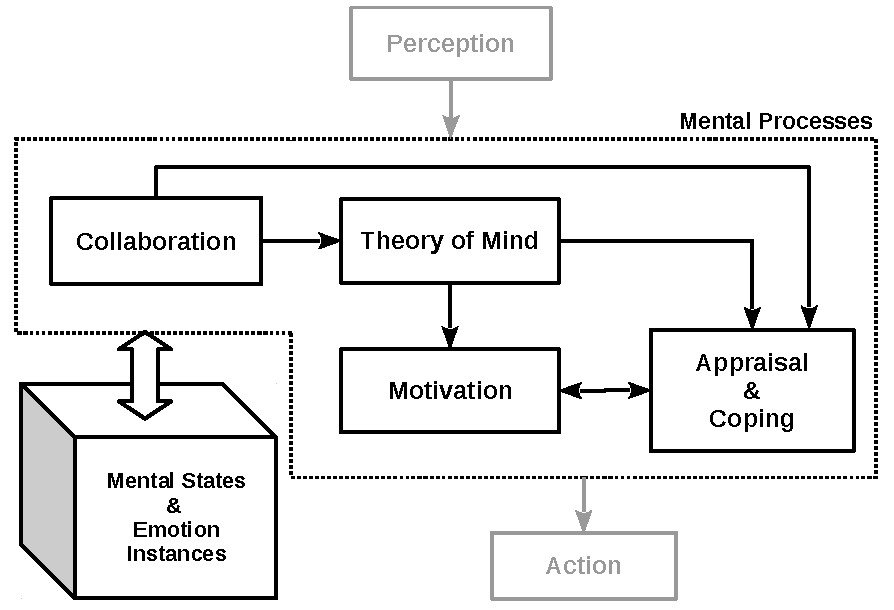
\includegraphics[scale=0.78]{figure/theory-general-croped.pdf}
  \caption{Roadmap of \textit{Affective Motivational Collaboration Theory}
  showing primary influences between processes.}
  \label{fig:theory}
\end{figure}

\section{Computational Framework}

\section{Walk Through Computational Examples}

\subsection{Agreeing on Shared Goal (Emotion-Awareness)}
\label{sec:wt-exp1}

\subsection{Agreeing on Shared Goal (Emotion-Ignorance)}

\subsection{Delegation of a Task (Emotion-Awareness)}

\subsection{Delegation of a Task (Emotion-Ignorance)}

\section{Conclusion and Future Work}

%\label{sec:2} ~\ref{sec:1}

%\paragraph{Paragraph headings} 


% For one-column wide figures use
%\begin{figure}
% Use the relevant command to insert your figure file.
% For example, with the graphicx package use
%  
\includegraphics{example.eps}
% figure caption is below the figure
%\caption{Please write your figure caption here}
%\label{fig:1}       % Give a unique label
%\end{figure}
%
% For two-column wide figures use
%\begin{figure*}
% Use the relevant command to insert your figure file.
% For example, with the graphicx package use
%  
\includegraphics[width=0.75\textwidth]{example.eps}
% figure caption is below the figure
%\caption{Please write your figure caption here}
%\label{fig:2}       % Give a unique label
%\end{figure*}
%



% For tables use
%\begin{table}
% table caption is above the table
%\caption{Please write your table caption here}
%\label{tab:1}       % Give a unique label
% For LaTeX tables use
%\begin{tabular}{lll}
%\hline\noalign{\smallskip}
%first & second & third  \\
%\noalign{\smallskip}\hline\noalign{\smallskip}
%number & number & number \\
%number & number & number \\
%\noalign{\smallskip}\hline
%\end{tabular}
%\end{table}


%\begin{acknowledgements}
%If you'd like to thank anyone, place your comments here
%and remove the percent signs.
%\end{acknowledgements}

% BibTeX users please use one of
%\bibliographystyle{spbasic}      % basic style, author-year citations
%\bibliographystyle{spmpsci}      % mathematics and physical sciences
%\bibliographystyle{spphys}       % APS-like style for physics
%\bibliography{}   % name your BibTeX data base

% Non-BibTeX users please use
\begin{thebibliography}{}
%
% and use \bibitem to create references. Consult the Instructions
% for authors for reference list style.
%
\bibitem{RefJ}
% Format for Journal Reference
Author, Article title, Journal, Volume, page numbers (year)
% Format for books
\bibitem{RefB}
Author, Book title, page numbers. Publisher, place (year)
% etc
\end{thebibliography}

\end{document}
% end of file template.tex

